\section{Algoritmi}\label{algoritmi}

\subsection{Notazione}\label{notazione}

La notazione utilizzata è la seguente:

\begin{itemize}
    \item \textit{user}: l'utente
    \item \textit{item}: l'oggetto
    \item \textit{rating}: valutazione/i
    \item $m$: numero di \textit{user}
    \item $n$: numero di \textit{item}
    \item $R$: l'insieme di tutti i \textit{rating}.
    \item $R_{train}$, $R_{test}$ e $\hat{R}$ indicano il set di addestramento, il set di test e l'insieme dei \textit{rating} previsti.
    \item $U$ : l'insieme di tutti gli \textit{user}. $u$ e $v$ indicano gli \textit{user}.
    \item $I$ : l'insieme di tutti gli \textit{item}. $i$ e $j$ indicano gli \textit{item}.
    \item $U_i$ : l'insieme di tutti gli \textit{user} che hanno valutato l'\textit{item} $i$.
    \item $U_{ij}$ : l'insieme di tutti gli \textit{user} che hanno valutato sia l'\textit{item} $i$ che l'\textit{item} $j$.
    \item $I_u$ : l'insieme di tutti gli \textit{item} valutati dallo \textit{user} $u$.
    \item $I_{uv}$ : l'insieme di tutti gli \textit{item} valutati sia dallo \textit{user} $u$ che dallo \textit{user} $v$.
    \item $r_{ui}$ : il \textit{rating} \textit{vero} dello \textit{user} $u$ per l'\textit{item} $i$.
    \item $\hat{r}_{ui}$ : il \textit{rating} \textit{stimato} dello \textit{user} $u$ per l'\textit{item} $i$.
    \item $b_{ui}$ : il \textit{rating} di base dello \textit{user} $u$ per l'\textit{item} $i$.
    \item $\mu$ : la media di tutti i \textit{rating}.
    \item $\mu_u$ : la media di tutti i \textit{rating} dati dallo \textit{user} $u$.
    \item $\mu_i$ : la media di tutti i \textit{rating} date all'\textit{item} $i$.
    \item $\sigma_u$ : la deviazione standard di tutti i \textit{rating} dati dallo \textit{user} $u$.
    \item $\sigma_i$ : la deviazione standard di tutte le valutazioni date all'\textit{item} $i$.
    \item $N_i^k(u)$ : i $k$ vicini più prossimi dello \textit{user} $u$ che hanno valutato l'\textit{item} $i$. Questo insieme è calcolato utilizzando una metrica di similarità.
    \item $N_u^k(i)$ : i $k$ vicini più prossimi dell'\textit{item} $i$ che sono valutati dallo \textit{user} $u$. Questo insieme è calcolato utilizzando una metrica di similarità.
\end{itemize}

\subsection{Algoritmi per Feedback Esplicito}\label{algoritmi-per-feedback-esplicito}

\subsubsection{SVD e SVD++}\label{matrix-factorization}

L'algoritmo SVD (\textit{singular value decomposition}), è stato reso popolare da Simon Funk durante la competizione \textit{the Netflix Prize} dimostrando come modelli di fattorizzazione matriciale sono superiori alle tecniche classiche basate su \textit{nearest neighbor}\ref{knn} per
la produzione di raccomandazioni.

I modelli di \textit{matrix factorization} mappano gli \textit{user} e gli \textit{item} in uno spazio latente comune di dimensione $k$, che rappresenta il numero di caratteristiche latenti. Ogni \textit{item} $i$ è associato a un vettore $q_i$ di dimensione $k$, che misura quanto l'\textit{item} possieda ciascuna di queste caratteristiche latenti. Per ogni \textit{user} $u$, invece, il vettore $p_u$ misura l'interesse dello \textit{user} per gli \textit{item}. Il numero di fattori è un iper-parametro dell'algoritmo.

In questo spazio, le interazioni tra \textit{user} e \textit{item} vengono modellate come prodotti scalari tra i rispettivi vettori. Lo spazio latente cerca di spiegare i \textit{rating} caratterizzando sia gli \textit{item} che gli textit{user} in base a fattori che vengono automaticamente dedotti. Ad esempio, se gli \textit{item} sono film, i fattori potrebbero appresentare il genere piuttosto che un altro (e.g. Azione contro Drama), profondità della trama o il concetto di "adatto ai bambini".

Il prodotto scalare risultante cattura l'interazione tra lo \textit{user} $u$ e l'\textit{item} $i$, che corrisponde all'interesse complessivo dello \textit{user} per le caratteristiche dell'\textit{item}. Il \textit{rating} finale viene ottenuto aggiungendo anche i predittori di base sopra menzionati, che dipendono solo dallo \textit{user} o dall'\textit{item}. Pertanto, un \textit{rating} viene predetto dalla regola~\cite{SVD_analysis}~\cite{Recommendation_book}:

\[
\hat{r}_{ui} = \mu + b_u + b_i + q_i^T p_u
\]

Dove:
\begin{itemize}
    \item $ \hat{r}_{ui} $ è il \textit{rating} previsto per
    l'\textit{item} $i$ da parte dello \textit{user} $u$.
    \item $ \mu $ è la media generale delle \textit{rating}.
    \item $ b_u $ e $ b_i $ sono i bias dello \textit{user} $u$ e dell'\textit{item} $i$ rispettivamente. Sono una sorta di correzione basata sull'effetto dello \textit{user} e dell'\textit{item}.
    \item $ q_i^T p_u $ è il prodotto interno tra i vettori latenti dello \textit{user} e dell'\textit{item}.
\end{itemize}

Se lo \textit{user} $u$ è sconosciuto, allora il bias $b_u$ e i fattori $p_u$ vengono considerati uguali a zero. Lo stesso vale per
l'\textit{item} $i$, con $b_i$ e $q_i$ anch'essi assunti uguali a zero.

Per apprendere i parametri del modello ($b_u$, $b_i$, $p_u$, $q_i$), si minimizza l'errore quadratico regolarizzato tra le \textit{rating} reali e quelle previste. L'errore quadratico è dato da:

\[
\text{min} \sum_{(u,i) \in K} \left (r_{ui} - \hat{r}_{ui})^2 + \lambda (\|q_i\|^2 + \|p_u\|^2 + b_u^2 + b_i^2 \right)
\]

Dove il primo termine è l'errore quadratico tra le \textit{rating} previste e reali e il secondo termine è la regolarizzazione, che penalizza valori troppo grandi per i parametri $b_u$, $b_i$, $p_u$, $q_i$ per evitare l'overfitting.

Per ottimizzare questi parametri, viene usata la \textit{stochastic gradient descent} (SGD), che aggiorna i parametri dopo ogni  esempio di training (ad esempio, per ogni \textit{rating} di un \textit{user}).

Per ogni \textit{rating} ($r_{ui}$) data, viene fatta una previsione ($\hat{r}_{ui}$), e l'errore di previsione associato ($e_{ui} = r_{ui} - \hat{r}_{ui}$) viene calcolato. Per un dato caso di addestramento ($r_{ui}$), modifichiamo i parametri spostandoci nella
direzione opposta al gradiente, ottenendo:

\begin{itemize}
    \item $b_u \leftarrow b_u + \gamma \cdot e_{ui}$
    \item $b_i \leftarrow b_i + \gamma \cdot e_{ui}$
    \item $q_i \leftarrow q_i + \gamma \cdot e_{ui} \cdot p_u$
    \item $p_u \leftarrow p_u + \gamma \cdot e_{ui} \cdot q_i$
\end{itemize}

dove $\gamma$ è il \textit{learning rate}. $\gamma$ e $\lambda$ sono iperparametri dell'algoritmo.

Queste formule vengono utilizzate per aggiornare i parametri durante l'addestramento del modello, in modo da ridurre l'errore tra le
\textit{rating} reali e quelle previste.

Per ottenere un ulteriore miglioramento, possono applicare $\gamma$ e $\lambda$ separati per i bias degli \textit{user}, i bias degli
\textit{item} e i fattori stessi~\cite{SVD_optimized}.

I punti di forza dell'algoritmo sono:

\begin{itemize}
    \item semplicità: l'algoritmo SVD è relativamente semplice da comprendere e implementare.
    \item riduzione della dimensionalità: l'algoritmo permette di ridurre la dimensione del problema mappando sia gli \textit{user} che gli \textit{item} in uno spazio latente di dimensione inferiore, gestendo la sparsità delle matrici. Funziona molto bene quando la matrice delle valutazioni è abbastanza completa. \item caratteristiche latenti: identifica strutture sottostanti che non sono immediatamente evidenti.
\end{itemize}

L'algoritmo soffre anche di diverse problematiche:

\begin{itemize}
    \item problemi con la sparsità: può produrre raccomandazioni imprecise quando la matrice delle valutazioni è troppo sparsa, perché la decomposizione non riesce a estrarre informazioni significative. 
    \item non tiene conto di informazioni aggiuntive: non considera altri fattori come informazioni temporali, contenuti aggiuntivi sugli \textit{item} o preferenze esplicite/implicite dell'utente che non sono registrati nella matrice.
    \item computazionalmente costosa: la decomposizione di una matrice grande è costosa in termini di tempo e risorse.
    \item overfitting: se non adeguatamente regolarizzato si rischia l'overfitting.
\end{itemize}

La precisione delle previsioni può essere migliorata considerando anche il feedback implicito, che fornisce un'indicazione aggiuntiva delle preferenze degli \textit{user}. Questo è particolarmente utile per gli \textit{user} che hanno fornito molto più feedback implicito che esplicito. Anche nei casi in cui il feedback implicito indipendente è assente, è possibile catturare un segnale significativo tenendo conto degli \textit{item} che gli \textit{user} hanno valutato, indipendentemente dal valore del \textit{rating}. Ciò ha portato a diversi metodi (\textit{Asymmetric-SVD}, \textit{SVD++}, \textit{SVD\_KNN}, ecc.~\cite{SVD++, SVD_KNN}) che modellano il fattore \textit{user} in base agli \textit{item} valutati. Il metodo \textit{SVD++} ha dimostrato di offrire una precisione superiore rispetto a \textit{SVD}.

Viene aggiunto un secondo set di fattori degli \textit{item}, che collega ogni \textit{item} $i$ a un vettore di fattori $y_i$ di dimensione $k$. Questi nuovi fattori vengono utilizzati per caratterizzare gli \textit{user} in base al set di \textit{item} che hanno valutato. La nuova predizione si calcola come segue:

\[
\hat{r}_{ui} = \mu + b_u + b_i + q_i^T \left(p_u + |I_u|^{\frac{1}{2}} \sum_{j \in I_u} y_j \right)
\]

Ora, un \textit{user} $u$ viene modellato come $p_u + |I_u|^{\frac{1}{2}} \sum_{j \in I_u} y_j$, mentre la parte $\sum_{j \in I_u} y_j$ rappresenta i feedback impliciti. Poiché i vettori $y_j$ sono centrati intorno a zero grazie alla regolarizzazione $|I_u|^{\frac{1}{2}}$, la varianza rispetto all'intervallo di valori osservati $|I_u|$ viene stabilizzata.

I parametri del modello vengono determinati minimizzando la funzione di errore quadratico regolarizzato, utilizzando sempre \textit{stochastic gradient descent}. Si itera su tutti i \textit{rating}:

\begin{itemize}
  \item $b_u \leftarrow b_u + \gamma \cdot (e_{ui} - \lambda \cdot b_u)$
  \item $b_i \leftarrow b_i + \gamma \cdot (e_{ui} - \lambda \cdot b_i)$
  \item $q_i \leftarrow q_i + \gamma \cdot \left( e_{ui} \cdot \left( p_u + |I_u|^{-\frac{1}{2}} \sum_{j \in I_u} y_j \right) - \lambda \cdot q_i \right)$
  \item $p_u \leftarrow p_u + \gamma \cdot (e_{ui} \cdot q_i - \lambda \cdot p_u)$
  \item $\forall j \in I_u: \quad y_j \leftarrow y_j + \gamma \cdot \left( e_{ui} \cdot |I_u|^{-\frac{1}{2}} \cdot q_i - \lambda \cdot y_j \right)$
\end{itemize}



È possibile introdurre diversi tipi di feedback implicito nel modello simultaneamente, utilizzando set aggiuntivi di fattori degli \textit{item}.

I punti di forza dell'algoritmo sono:

\begin{itemize}
    \item miglioramento della personalizzazione: SVD++ è un miglioramento significativo rispetto a SVD, poiché prende in considerazione anche l'influenza degli \textit{item} che lo \textit{user} ha già valutato nel termine $\sum_{j \in I_u} y_j$, il che lo rende molto più sensibile alle preferenze individuali dello \textit{user}.
    \item migliore gestione della sparsità: poiché SVD++ tiene conto dei feedback impliciti, riesce a fare previsioni migliori anche quando la matrice delle valutazioni è sparsa.
    \item previsioni più accurate: i feedback impliciti aiutano a produrre previsioni più accurate, soprattutto in scenari dove gli \textit{user} hanno interagito con più \textit{item}.
\end{itemize}

L'algoritmo soffre anche di diverse problematiche:

\begin{itemize}
    \item complessità computazionale maggiore: la necessità di aggiornare $y_i$ aumenta il carico computazionale.
    \item richiede più dati: poiché prende in considerazione anche i feedback impliciti, ha bisogno di un numero maggiore di dati per generare previsioni precise.
    \item overfitting: SVD++ è più propenso a overfitting su dataset piccoli.
\end{itemize}


\subsubsection{KNN}\label{knn}

\subsubsection{CoClustering}\label{coclustering}

La soluzione proposta da Thomas George e Srujana Merugu~\cite{Co-Clustering} utilizza il \textit{co-clustering}. Questa tecnica viene utilizzata per raggruppare simultaneamente due entità in un dataset. Nel caso di un sistema di \textit{recommendation} basato su \textit{collaborative filtering}, l'obiettivo è trovare gruppi di \textit{user} simili e gruppi di \textit{item} simili. Il co-clustering cerca di partizionare simultaneamente le righe (\textit{user}) e le colonne (\textit{item}) della matrice dei \textit{rating} in modo tale che gli \textit{user} all'interno dello stesso co-cluster abbiano comportamenti di valutazione simili e \textit{item} all'interno dello stesso co-cluster siano valutati in modo simile dagli \textit{user} del co-cluster. Il numero di cluster è da definire a priori sia per gli \textit{user} che per gli \textit{item}. Il processo di co-clustering è simile al clustering tradizionale, ma mentre nel clustering classico si raggruppa solo per righe o colonne, nel co-clustering si raggruppano contemporaneamente. 

L'algoritmo, nella fase di inizializzazione, assegna casualmente i co-cluster a \textit{user} e \textit{item}. Durante l'esecuzione i co-cluster vengono aggiornati iterativamente, per cercare di migliorare la qualità del raggruppamento, alternando tra il raggruppamento degli \textit{user} e degli \textit{item} fino a convergenza. Una volta che i co-cluster sono definiti si può calcolare la media dei \textit{rating} all'interno di ciascun co-cluster. $ \overline{C_{ui}} $ rappresenta la media dei \textit{rating} all'interno del co-cluster che contiene lo \textit{user} $ u $ e l'\textit{item} $ i $. In altre parole, è il \textit{rating} medio tra gli \textit{user} e gli \textit{item} che appartengono allo stesso co-cluster.

Si può quindi definire la predizione come

\[
\hat{r}_{ui} = \overline{C_{ui}} + (\mu_u - \overline{C_u}) + (\mu_i - \overline{C_i})
\]

dove $\overline{C_u}$ è la media dei \textit{rating} del cluster di $u$ e $\overline{C_i}$ è la media dei \textit{rating} del cluster di $i$. $ \mu_u - \overline{C_u} $ e $ \mu_i - \overline{C_i} $ vengono definiti \textit{bias}. Se: 
\begin{itemize}
  \item \textit{user} mancante: la previsione è $ \overline{C_i} $
  \item \textit{item} mancante: la previsione è $ \overline{C_u} $
  \item se sia \textit{user} che \textit{item} sono mancanti: la previsione è $ \mu $, la media generale dei rating.
\end{itemize}

I punti di forza dell'algoritmo sono:

\begin{itemize}
  \item Scalabilità: l'algoritmo di co-clustering può essere facilmente parallelizzato, il che lo rende adatto per sistemi di \textit{recommendation} con grandi quantità di dati.
  \item Gestione dei comportamenti complessi: la previsione tiene conto sia del co-cluster, che considera simultaneamente i raggruppamenti di \textit{user} e \textit{item}, sia dei cluster singoli per \textit{user} e \textit{item}. Questo permette di considerare diversità e similarità sia individualmente che insieme, migliorando le previsioni.
  \item Gestione semplice degli aggiornamenti: quando nuovi dati sono aggiunti al sistema, è possibile aggiornare solo i co-cluster rilevanti senza dover ricalcolare tutto da zero. Questo è particolarmente utile per scenari dinamici e sistemi in tempo reale.
  \item Gestione della sparsità: poiché l'algoritmo raggruppa \textit{user} e \textit{item} simili, riduce l'effetto della sparsità permettendo di migliorare la qualità delle previsioni anche quando i dati disponibili sono pochi o incompleti.
\end{itemize}

L'algoritmo soffre anche di diverse problematiche:

\begin{itemize}
  \item Sensibilità ai co-cluster: la qualità delle previsioni dipende molto dal numero di co-cluster scelto e dalla loro qualità. Se il numero di co-cluster è troppo basso, il modello potrebbe non riuscire a catturare le complessità dei dati e fare previsioni imprecise. Se il numero è troppo alto, il modello potrebbe overfittare i dati di addestramento, riducendo la sua generalizzazione. Inoltre, se i co-cluster non sono ben definiti, il modello potrebbe produrre previsioni inaccurate. La scelta iniziale dei co-cluster è fondamentale. Una soluzione è quella di utilizzare l'algoritmo \textit{K-means} per definire la posizione iniziale dei cluster.
  \item Bias del co-cluster: $ \mu_u - \overline{C_u} $ e $ \mu_i - \overline{C_i} $ potrebbero non essere sempre utili in tutte le situazioni. Alcuni \textit{user} o \textit{item} potrebbero avere comportamenti che non sono ben rappresentati dai co-cluster e il modello potrebbe non adattarsi bene a queste situazioni. Ad esempio, \textit{user} che tendono a esprimere \textit{rating} bassi potrebbero non essere gestiti correttamente.
  \item Alto costo computazionale iniziale: l'algoritmo ha un alto costo computazionale durante la fase di addestramento, soprattutto con set di dati molto grandi. Anche se è scalabile, l'ottimizzazione del processo di clustering e la ricerca del numero ottimale di co-cluster richiedono parecchia computazione.
  \item Difficoltà di interpretazione: il co-clustering fornisce gruppi di \textit{user} e \textit{item} che potrebbero non essere sempre facili da interpretare o da analizzare in modo intuitivo.
\end{itemize}

Il costo computazionale per l'addestramento è $ O(W^{\text{glob}} + mkl + nkl) $ dove $ W^{\text{glob}} $ corrisponde al numero di valori diversi da 0 nella matrice in input , $l$ corrisponde al numero di cluster per gli \textit{user} e $k$ corrisponde al numero di cluster per gli \textit{item}.

Per il calcolo della predizione, il costo è $O(1)$, in quanto si tratta di operazioni media e il calcolo dei bias.

Per l'aggiornamento quando un nuovo \textit{rating} viene aggiunto o un nuovo \textit{user}/\textit{item} entra nel sistema, l'algoritmo non ricalcola tutto da zero. Invece, utilizza un aggiornamento incrementale parziale, che si basa sull'aggiornamento delle medie delle matrici:

\begin{itemize}
  \item Se il nuovo \textit{rating} riguarda un \textit{user} e un \textit{item} esistenti si aggiornano direttamente le medie.
  \item Se l'\textit{user} o l'\textit{item} è nuovo, viene assegnato temporaneamente a un co-cluster globale di transizione. Le medie vengono aggiornate e, durante la successiva esecuzione dell'algoritmo, il nuovo \textit{user}/\textit{item} viene riassegnato ai co-cluster regolari.
\end{itemize}

L'aggiornamento ha quindi costo pari a $O(1)$.


\subsubsection{Slope One}\label{slopeone}

L'algoritmo Slope One, introdotto da Daniel Lemire e Anna Maclachlan~\cite{SlopeOne}, è una delle soluzioni più semplici ed efficienti di collaborative filtering.
%
Le caratteristiche che lo rendono un ottimo algoritmo per la \textit{recommendation} sono:
\begin{itemize}
    \item la semplicità e facilità di implementazione
    \item velocità di calcolo: come verrà presentato più avanti alcuni valori calcolati possono essere salvati e aggiornati all'occorrenza rendendo il calcolo molto più veloce
    \item scalabilità: l'algoritmo può essere abbastanza efficace su dataset di dimensioni moderate, soprattutto se si utilizzano tecniche di compressione dei dati
    \item facilità di interpretazione
\end{itemize}
%
Viene proposto un predittore basato su differenze di \textit{rating} lineari che ha un'efficienza $O(nm)$ per predizione e $O(mn^2)$ per addestramento.

L'algoritmo si basa sulla differenza media tra le valutazioni di due \textit{item} per predire il \textit{rating} mancante. La differenza media dei \textit{rating} di due \textit{item} $i$ e $j$ viene calcolata come:

\[
    \text{dev}(i, j) = \frac{1}{|U_{i,j}|} \sum\limits_{u \in U_{i,j}} (r_{u,i} - r_{u,j})
\]

La matrice simmetrica definita da $\text{dev}(i, j)$ può essere computata una volta e aggiornata velocemente quando vengono aggiunti nuovi dati.

La predizione viene dunque calcolata come:

\[
    \hat{r}_{ui} = \mu_u + \frac{1}{|R_i(u)|} \sum\limits_{j \in R_i(u)} \text{dev}(i, j)
\]

dove:

\begin{itemize}
    \item $R_j = \{ i \mid i \in S(u), i \neq j, |S_{j,i}(\chi)| > 0 \}$ è l'insieme degli \textit{item} rilevanti
    \item $S(u)$ è il sottoinsieme degli item valutati dallo \textit{user} $u$
    \item $S_{j,i}(\chi)$ è l'insieme di tutte le valutazioni $u$ nel dataset $\chi$ che contengono gli \textit{item} $i$ e $j$
\end{itemize}

\begin{figure}[H]
    \centering
    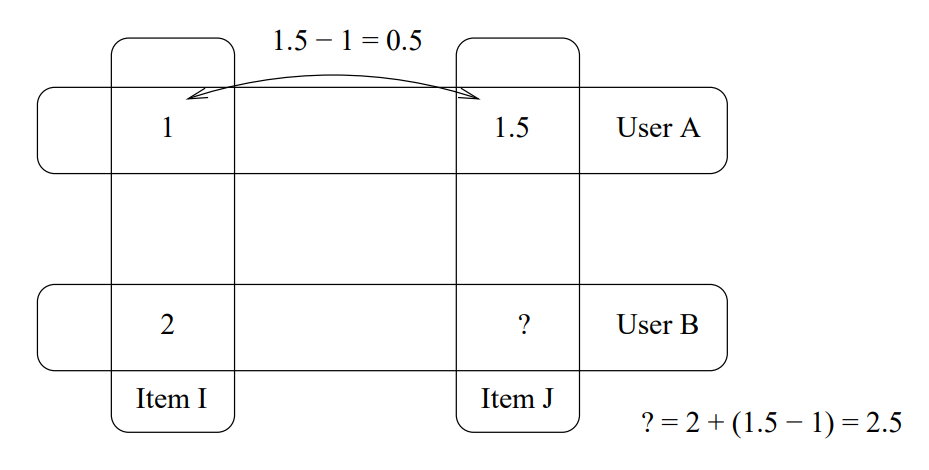
\includegraphics[keepaspectratio]{figures/algorithms/slope_one.PNG}
    \caption{Base dello schema Slope One: le valutazioni dello \textit{user} A di due \textit{item} e la valutazione  dello \textit{user} B di un \textit{item} comune vengono utilizzate per prevedere la valutazione sconosciuta dello \textit{user}.}
    \label{fig:slopeone}
\end{figure}

L'algoritmo soffre anche di diverse problematiche:
\begin{itemize}
    \item sparsità dei dati: le formule presentate prima sono approssimate considerando un dataset non sparso. Nel caso di matrici molto sparse l'algoritmo non sarà in grado di fare previsioni accurate
    \item scalabilità limitata su dataset molto grandi: la memoria necessaria per memorizzare le differenze medie dei \textit{rating} può aumentare rapidamente
    \item non tiene conto nè di personalizzazioni per \textit{user} 
    \item difficoltà a gestire grandi variazioni nelle valutazioni degli utenti
\end{itemize}

L'approccio può essere esteso a modelli ponderati e versioni più avanzate, come per esempio \emph{Weighted Slope One}, che pesa le differenze di \textit{rating} in base alla frequenza di coppie di \textit{item} valutati, e \emph{Regression-based Slope One}, che introduce funzioni non lineari per migliorare la precisione delle previsioni.

\subsubsection{Evaluation esplicita}\label{evaluation-esplicita}

\subsubsection{Algoritmi per Feedback Implicito}\label{algoritmi-per-feedback-implicito}

\subsubsection{ALS (Alternating Least Squares)}\label{als-alternating-least-squares}

\subsubsection{BPR (Bayesian Personalized Ranking)}\label{bpr-bayesian-personalized-ranking}

\subsubsection{LMF (Logistic Matrix Factorization)}\label{lmf-logistic-matrix-factorization}

\subsubsection{Evaluation implicita}\label{evaluation-implicita}

\subsubsection{Algoritmi per la Similarità Item-Item}\label{algoritmi-per-la-similarita-item-item}

\subsubsection{Algoritmi Ibridi}\label{algoritmi-ibridi}

\subsubsection{LightFM}\label{lightfm}

\subsubsection{Introduzione a Modelli di Deep Learning}\label{introduzione-a-modelli-di-deep-learning}
